\documentclass[UTF8,a4paper]{article}
\usepackage{array}
\usepackage{amsmath}
\usepackage{listings}
\usepackage{graphicx}
\usepackage{subcaption}
\usepackage{color} %red, green, blue, yellow, cyan, magenta, black, white
\definecolor{mygreen}{RGB}{28,172,0} % color values Red, Green, Blue
\definecolor{mylilas}{RGB}{170,55,241}
\usepackage{geometry}
\geometry{left=2.0cm,right=2.0cm,top=2.0cm,bottom=2.0cm}

\renewcommand{\theequation}{\arabic{section}.\arabic{equation}}
\renewcommand{\thefigure}{\arabic{section}.\arabic{figure}}
\renewcommand{\thetable}{\arabic{section}.\arabic{table}}
\makeatletter
\@addtoreset{equation}{section}
\@addtoreset{figure}{section}
\@addtoreset{table}{section}
\makeatother

\title{Digital Image Processing 2017fall \\ Project Report }
\author{Name: Wang Yiqing \\ Student Number: 515 030 910 456 \\ Email: WangYiqing\_2015@sjtu.edu.cn}
\date{2017-12-10}

\begin{document}
\maketitle

\clearpage
\tableofcontents

\clearpage

\lstset{language=Matlab,%
    %basicstyle=\color{red},
    frame=single, %设置边框格式
    breaklines=true,%
    morekeywords={matlab2tikz},
    keywordstyle=\color{blue},%
    morekeywords=[2]{1}, keywordstyle=[2]{\color{black}},
    identifierstyle=\color{black},%
    stringstyle=\color{mylilas},
    commentstyle=\color{mygreen},%
    showstringspaces=false,%without this there will be a symbol in the places where there is a space
    numbers=left,%
    numberstyle={\tiny \color{black}},% size of the numbers
    numbersep=9pt, % this defines how far the numbers are from the text
    emph=[1]{for,end,break},emphstyle=[1]\color{blue}, %some words to emphasise
    %emph=[2]{word1,word2}, emphstyle=[2]{style},    
}

\section{Project 1 - Histogram Equalization}

\subsection{Project Proposal}
In this project we implement histogram equalization. First, plot the histogram of an image, then implement histogram equalization and display the equalized image and histogram. Test images are \emph{Fig1.jpg, Fig2.jpg}.

\subsection{Preliminaries}
Let $r$ denote the intensity of a pixel in the original image and $r \in [0,L-1]$. We consider a transformation \begin{equation}s=T(r) ~~~~ 0 \leq r \leq L-1 \end{equation} that produce an output intensity level $s$ for every pixel in the input image having intensity $r$. We assume that:
\\ \textbf{(a)} $T(r)$ is a monotonically increasing function in the interval $0 \leq r \leq L-1$; and \\
\textbf{(b)} $0 \leq T(r) \leq L-1$ for $r \in [0, L-1]$. \\
Condition \textbf{(a)} and \textbf{(b)} guarantee the existing of inverse function $r=T^{-1}(s)$ which is monotonically increasing. 
The central idea is that \emph{intensity levels of an image can be viewed as random variables in the interval $[0, L-1]$ and can be described by probability density function (PDF).} Let $p_r(r)$ and $p_s(s)$ to be the PDF of $r$ and $s$ respectively. Thus we can apply the basic result of probability theory that \emph{if $T(r)$ is differentiable over the range of interest, we have this below relationship between $p_r(r)$ and $p_s(s)$: }
\begin{equation} p_s(s)=p_r(r) \left| \frac{dr}{ds} \right| \label{equ:basicprob} \end{equation}
Then consider the cumulative distribution function(CDF) which is exactly used here as the transformation function $T(r)$ \begin{equation} s=T(r)=(L-1) \int_0^r p_r(w)dw  \label{equ:histEquTrans} \end{equation}
Now we are ready to prove the transformation really does the histogram equalization. Firstly, compute the derivatives. The last $=$ is from the assumption \textbf{(a)} stating the monotonically increasing.
\begin{equation} \frac{ds}{dr}=\frac{dT(r)}{dr}=(L-1)p_r(r) = \left| \frac{ds}{dr} \right| \end{equation}
Thus, substituting the result for Eq.\ref{equ:basicprob}, we get the desired result
\begin{equation} p_s(s) = p_r(r) \frac{1}{(L-1)p_r(r)} = \frac{1}{L-1} \end{equation}
which show $p_s(s)$ follows uniform distribution.

\subsection{Histogram equalization}
Histogram equalization on an image of size $M\times N$ is like a discrete version of the process in the preliminaries section. \begin{equation} p_r(r_k)=\frac{n_k}{MN} ~~~~~~ k=0,1,2,...,L-1  \end{equation} where $n_k$ is the number of pixels that have intensity $r_k$. The discrete form of Eq.\ref{equ:histEquTrans} is \begin{equation} s_k=T(r_k)=(L-1)\sum_{j=0}^k p_r(r_j)=\frac{L-1}{MN} \sum_{j=0}^k n_k ~~~~~~ k=0,1,2,...,L-1 \end{equation}
Based on these discrete form equation, I implement the matlab function and test them on \emph{Fig1.jpg, Fig2.jpg} and get the results listed in \ref{fig:result1} and \ref{fig:result2} respectively.
\begin{figure}[h!]
	\centering
	\begin{subfigure}[b]{0.45\linewidth}
		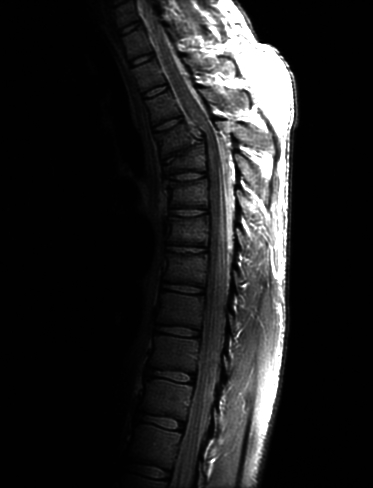
\includegraphics[width=\linewidth]{myfigure/p1/Fig1.jpg}
		\caption{}
		\label{fig:Fig1}
	\end{subfigure}
  	\begin{subfigure}[b]{0.45\linewidth}
		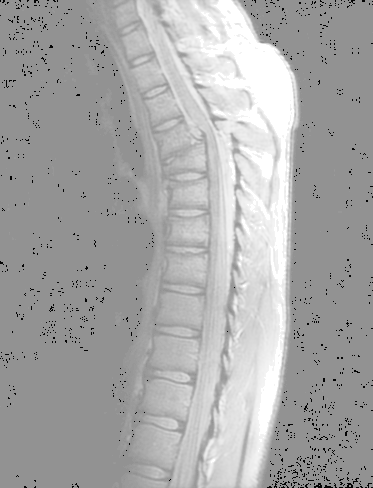
\includegraphics[width=\linewidth]{myfigure/p1/g1.png}
		\caption{}
		\label{fig:g1}
	\end{subfigure}
	\begin{subfigure}[b]{0.45\linewidth}
    	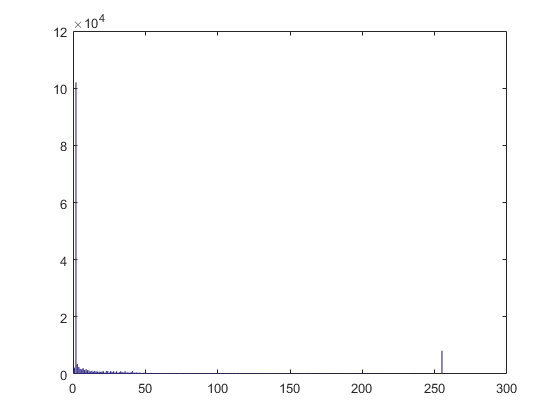
\includegraphics[width=\linewidth]{myfigure/p1/fbar1.png}
    	\caption{}
    	\label{fig:fbar1}
  	\end{subfigure}
	\begin{subfigure}[b]{0.45\linewidth}
    	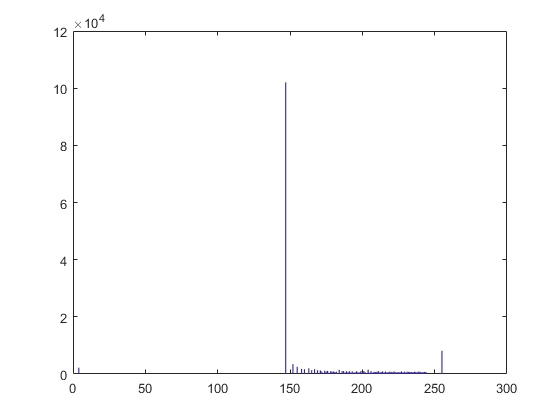
\includegraphics[width=\linewidth]{myfigure/p1/gbar1.png}
    	\caption{}
    	\label{fig:gbar1}
  	\end{subfigure}
  	\caption{Results of Fig1.jpg. (a)Original image. (b)Processed image after applying histogram equalization. (c)Histogram of original image. (d)Histogram of processed image.}
  	\label{fig:result1}
\end{figure}

\begin{figure}[h!]
	\centering
	\begin{subfigure}[b]{0.45\linewidth}
		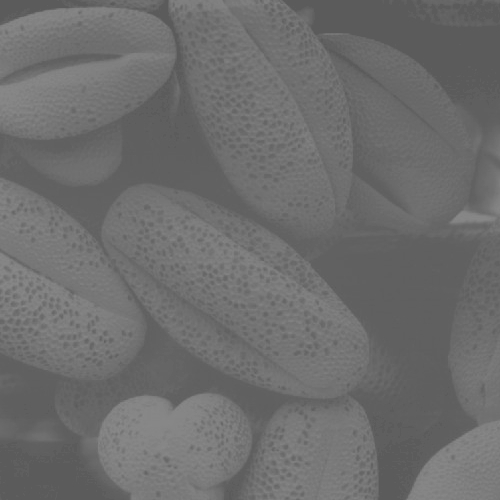
\includegraphics[width=\linewidth]{myfigure/p1/Fig2.jpg}
		\caption{}
		\label{fig:Fig2}
	\end{subfigure}
	\begin{subfigure}[b]{0.45\linewidth}
		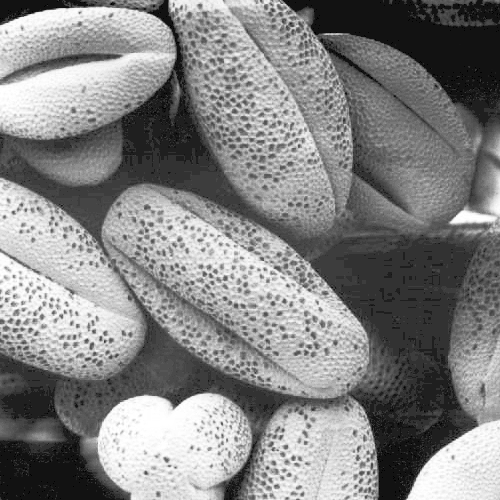
\includegraphics[width=\linewidth]{myfigure/p1/g2.png}
		\caption{}
		\label{fig:g2}
	\end{subfigure}
	\begin{subfigure}[b]{0.45\linewidth}
    	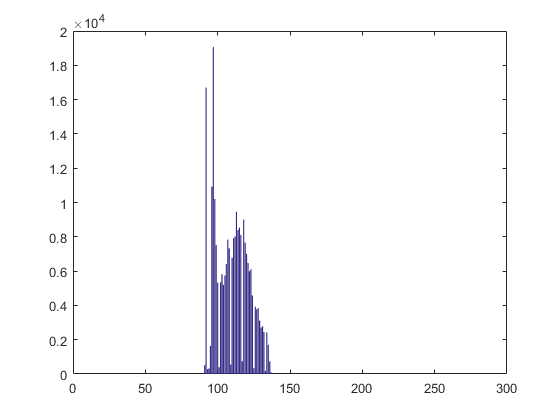
\includegraphics[width=\linewidth]{myfigure/p1/fbar2.png}
    	\caption{}
    	\label{fig:fbar2}
  	\end{subfigure}
	\begin{subfigure}[b]{0.45\linewidth}
    	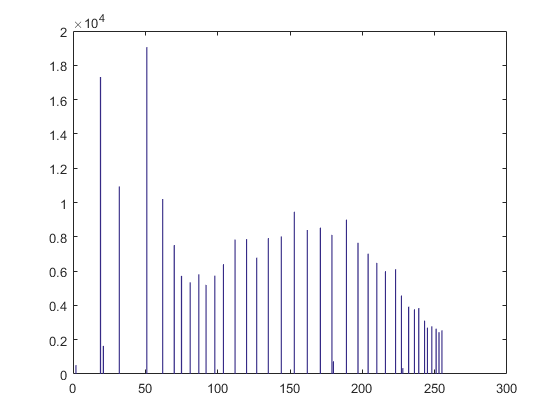
\includegraphics[width=\linewidth]{myfigure/p1/gbar2.png}
    	\caption{}
    	\label{fig:gbar2}
  	\end{subfigure}
  	\caption{Results of Fig2.jpg. (a)Original image. (b)Processed image after applying histogram equalization. (c)Histogram of original image. (d)Histogram of processed image.}
  	\label{fig:result2}
\end{figure}

\clearpage

\subsection{Discussion}
We can see that histograms are quite different from continuous functions because there are gaps between each horizontal value. So the histogram of the equalized image is like a sparse version of the original image. The result of Fig2(low contrast ratio) shows an increasing on contrast ratio and it's more useful than the original result. However, Fig1(high contrast ratio) is not a good example of histogram equalization. The affect is just like a intensity transition. We can simply draw a not so serious conclusion that histogram equalization is useful for images with low contrast ratio but not for images with high contrast ratio.

\subsection{Implementation}
There is some key part of my implementation.
\lstset{language=Matlab}
\begin{lstlisting}
function [x, y] = histShow( imgf )
%HISTSHOW display the histogram graph of the imgf
% x - the horizontal axis of histogram, 
% y - the vertical axis of histogram
g = imgf(:) + 1;
n = length(g);
x = (1 : 256);
y = zeros(1, 256);
for i = (1 : n)
    y(g(i)) = y(g(i)) + 1;
end

end

function [ imgg ] = histEqual( imgf )
%HISTEQUAL 
%   
[x, y] = histShow(imgf);
T = zeros(1, 256);
a = 0;
g = imgf(:);
n = length(g);
for i = (1 : 256)
    T(i) = a + y(i);
    a = T(i);
end
T = round(255 * T / n);
for i = (1 : n)
    g(i) = T(g(i)+1);
end
imgg = reshape(g, size(imgf));

end
\end{lstlisting}





\section{Project 3 - Filtering in Frequency Domain}

\subsection{Project Proposal}
Implement the ideal, Butterworth and Gaussian lowpass and highpass filters and the results under different parameters using the image character\_test\_pattern.tif

\subsection{Preliminaries}
\subsubsection{Summary of Fourier transform properties}

\begin{table}[h]
	\caption{Summary of useful formulas.}
	\centering
	\begin{tabular}{|l|m{0.6\columnwidth}|}\hline
		Name & Expression(s) \\ \hline
		1D FT & \begin{equation}F(u)=\int_{-\infty}^\infty f(t)e^{-j2 \pi ut}dt \end{equation} \\ 
		1D IFT & \begin{equation}f(t)=\int_{-\infty}^\infty F(u)e^{j2 \pi ut}du\end{equation} \\
		1D DFT & \begin{equation}F(u)=\sum_{t=0}^{M-1}f(t)e^{-j2\pi ut/M} \end{equation} \\
		1D IDFT & \begin{equation}f(t)=\frac{1}{M}\sum_{u=0}^{M-1}F(u)e^{j2\pi ut/M}\end{equation} \\
		2D FT & \begin{equation} F(u,v)=\int_{-\infty}^\infty \int_{-\infty}^\infty f(x,y)e^{-j2 \pi (ux+vy)}dxdy \end{equation} \\
		2D DFT & \begin{equation} F(u,v)= \sum_{x=0}^{M-1}\sum_{y=0}^{N-1} f(x,y)e^{-j2\pi (ux/M+vy/N)}\end{equation} \\
		2D IDFT & \begin{equation} f(x,y) = \frac{1}{MN}\sum_{u=0}^{M-1}\sum_{v=0}^{N-1]}F(u,v)e^{j2\pi(ux/M+vy/N)} \end{equation} \\
		Power spectrum & \begin{equation} P(u,v)=|F(u,v)|^2 \end{equation} \\
		\hline
	\end{tabular}
\end{table}

\subsubsection{Steps for filtering in the frequency domain}
\begin{enumerate}
	\item Given an input image $f(x,y)$ of size $M\times N$, obtain the padding parameters $P=2M$ and $Q=2N$.Form a padded image, $f_p(x,y)$, of size $P\times Q$ by appending zeros.
	\item Multiply $f_p(x,y)$ by $(-1)^{x+y}$ to center its transform.
	\item Compute the DFT, $F(u,v)$ of the image from centered padded image.
	\item Generate a real, symmetric filter function $H(u,v)$ of size $P \times Q$ with center at coordinates $(P/2, Q/2)$. Form the product $G(u,v)=H(u,v)F(u,v)$.
	\item Obtain the precessed image: $g_p(x,y)=\left\{ \text{real}\left[\ \mathcal{F}^{-1}[G(u,v)] \right] \right\}(-1)^{x+y}$ where the real part is selected in order to ignore parasitic complex components resulting from computational inaccuracies.
	\item Obtain the final processed result, $g(x,y)$, by extracting the top left $M\times N$ quadrant of $g_p(x,y)$
\end{enumerate}


\subsection{Image Smoothing Using Frequency Domain Filters}
Edges and other sharp intensity transitions such as noise in an image contribute significantly to the high-frequency content of its Fourier transform. Hence, smoothing is achieved in the frequency domain by high-frequency attenuation.
\subsubsection{Ideal lowpass filters}
\emph{Ideal lowpass filters (ILPF)} is very sharp as it is specified by the function 
\begin{equation}
H(u,v) = \left \{ \begin{array}{rcl}
1 & \text{if $D(u,v)\leq D_0$} \\
0 & \text{otherwise}
\end{array} \right.
\end{equation}
where $D_0$ is a positive constant and $D(u,v)$ is the distance between  $(u,v)$ in frequency domain and the center of the frequency rectangle; that is \begin{equation} D(u,v) = \left[ (u-P/2)^2+(v-Q/2)^2 \right]^{1/2} \end{equation} 
One way to establish a set of standard cutoff frequency loci is to compute circles that enclose specified amounts of total image power $P_T$. \begin{equation} P_T=\sum_{u=0}^{P-1}\sum_{v=0}^{Q-1}P(u,v) \end{equation}
The percentage of power enclosed by the circle of radius $D_0$ with origin at the center of the frequency rectangle is \begin{equation} \alpha=100\left[\ \sum_u\sum_vP(u,v)/P_T \right] ~~~~ \text{(u,v) is inside the circle}\end{equation}


\section{Project 8 - Morphological Processing}

\subsection{Project Proposal}
Implement the \emph{"Opening by reconstruction", "Filling holes" and "Border clearing"} operations on textbook \emph{chapter 9.5}. The task is to reproduce the results in \emph{Figure 9.29, 9.31 and 9.32}.

\subsection{Preliminaries}
\subsubsection{Basic morphological operations}
Morphology offers a unified and powerful approach to numerous image processing problem. These operations defined based on set theory. In this project we consider that morphological operations are conducted on binary images (preprocessing is required for gray-level images). The below table describes the basic widely used morphological processing.
\begin{table}[h]
	\caption{Summary of basic morphological operations.}
	\centering
	\begin{tabular}{|l|l|m{0.45\columnwidth}|}\hline
		Operation & Equation & Comments\\ \hline
		Translation & $(B)_z=\{w|w=b+z, ~ b \in B \}$ & Translation the origin of $B$ to point $z$.\\
		Reflection & $\hat{B}=\{w|w=-b, ~ b \in B\}$ & Reflects all elements of B about the origin of this set.\\
		Complement & $A^c=\{ w|w \notin A \}$ & Set of points not in $A$.\\
		Difference & $A-B=\{ w|w \in A, w \notin B\}$ & Set of points that belong to $A$ but not to $B$.\\
		Dilation & $A \oplus B=\left\{ z|(\hat{B}_z) \cap A \neq \emptyset \right\}$ & Expands the boundary of $A$.\\
		Erosion & $A \ominus B=\left\{ z|(B)_z \subseteq A \right\}$ & Contracts the boundary of $A$.\\
		Opening & $A \circ B=(A\ominus B)\oplus B $ & Smoothes contours, breaks narrow isthmuses, and eliminates small islands and sharp peaks.\\
		Closing & $A \bullet B=(A\oplus B)\ominus B $ & Smoothes contours, fuses narrow breaks and long thin gulfs and eliminates small holes.\\
		Hit-or-miss transform & $A \otimes B=(A\ominus B_1)\cap(A^c\ominus B_2)$ & The set of pints at which, simultaneously $B_1$ found a hit in $A$ and $B_2$ found a match in $A^c$.\\ \hline
	\end{tabular}
\end{table}

\subsubsection{Morphological restoration}
With the basic operations, we can discuss a powerful morphological transformation \emph{morphological restoration} that involves two images and a structuring element. One image, the \emph{marker}, contains the starting points for the transformation. The other image, the \emph{mask}, constrains the transformation. \\
\subsubsection*{Geodesic dilation and erosion}
Geodesic dilation and erosion are the central concepts to morphologic reconstruction. Let $F$ denote the maker and $G$ denote the mask and $F \subseteq G$. The \emph{geodesic dilation} of size 1 of the marker with respect to the mask, denoted by $D_G^(1)(F)$, is defined as 
\begin{equation} D_G^{(1)}(F)=(F\oplus B) \cap G \end{equation}
The geodesic dilation of size $n$ of $F$ with resplect to $G$ is defined as 
\begin{equation} D_G^{(n)}(F)=D_G^{(1)} \left[ D_G^{(n-1)}(F) \right]\end{equation}
with $D_G^{(0)}(F)=F$. Similarly, the \emph{geodesic erosion} of size 1 of marker $F$ with respect to mask $G$ is defined as 
\begin{equation} E_G^{(1)}(F)=(F\ominus B) \cup G \end{equation}
The geodesic erosion of size $n$ of $F$ with respect to $G$ is defined as
\begin{equation} E_G^{(n)}(F)=E_G^{(1)} \left[ E_G^{(n-1)}(F) \right]\end{equation}
with $E_G^{(0)}(F)=F$. Geodesic dilation and erosion are duals with respect to set complementation. \\
\subsubsection*{Morphological reconstruction by dilation and by erosion}
\emph{Morphological reconstruction by dilation of a mask $G$ from a marker $F$}, denoted $R_G^D{F}$ is defined \begin{equation}R_G^D(F)=D_G^{(k)}(F)\end{equation} with $k$ such that \begin{equation}D_G^{(k)}(F)=D_G^{(k+1)}(F)\end{equation} \emph{Morphological reconstruction by erosion of mask $G$ from a marker $F$}, denoted $R_G^E(F)$ is defined \begin{equation}R_G^E(F)=E_G^{(k)}(F)\end{equation} with $k$ such that \begin{equation}E_G^{(k)}(F)=E_G^{(k+1)}(F)\end{equation}


\subsection{Task-1 Opening by reconstruction}
The opening by reconstruction of size $n$ of an image $F$ is defined as the reconstruction by dilation of $F$ from the erosion of size $n$ of $F$; that is \begin{equation}O_R^{(n)}(F)=R_F^D \left[ (F\ominus nB) \right]\end{equation} where $(F\ominus nB)$ indicates $n$ erosions of $F$ by $B$. \\
Figure \ref{fig:0929a} is the original image for this task. We are interested in extracting the characters that contain long, vertical strokes. The origin image is of size $918 \times 2018$ pixels. The approximate average height of the tall characters is 50 pixels. Thus we use a structuring element of size $51 \times 1$ pixels to erode the original image. The erosion image is shown in Figure \ref{fig:0929b}. For comparison, Figure \ref{fig:0929c} shows the opening of Figure \ref{fig:0929a} with the same structuring element. Using erosion image (b) as the marker and the original image (a) as mask, we restored the characters containing long vertical strokes accurately via opening by reconstruction. This result is displayed in Figure \ref{fig:0929d}. \\

\begin{figure}[h!]
	\centering
	\begin{subfigure}[b]{0.45\linewidth}
		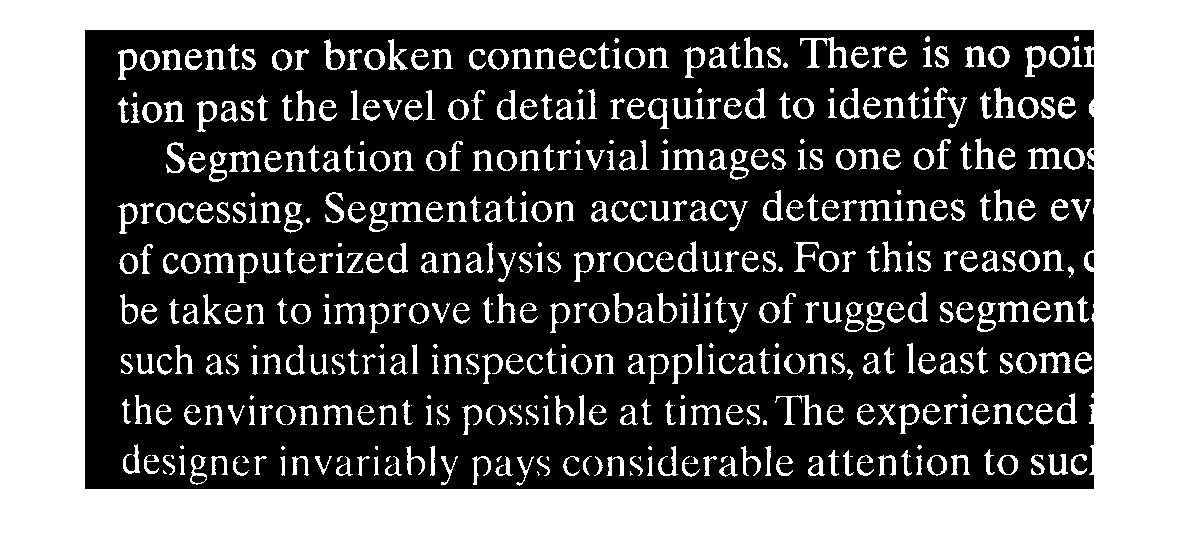
\includegraphics[width=\linewidth]{myfigure/p8/fig0929(a).png}
		\caption{}
		\label{fig:0929a}
	\end{subfigure}
	\begin{subfigure}[b]{0.45\linewidth}
    	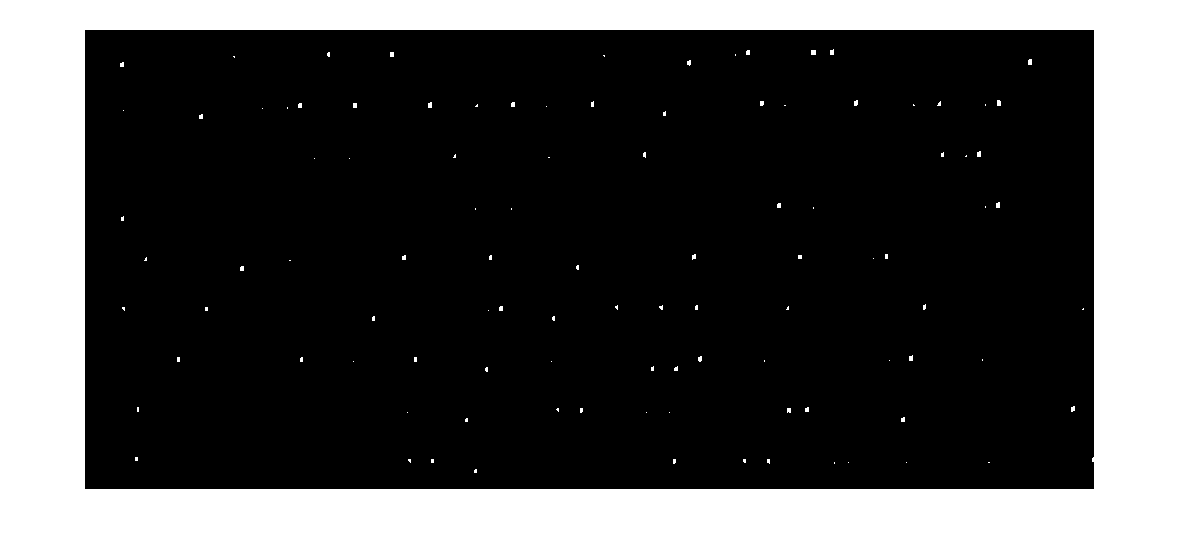
\includegraphics[width=\linewidth]{myfigure/p8/fig0929(b).png}
    	\caption{}
    	\label{fig:0929b}
  	\end{subfigure}
  	\begin{subfigure}[b]{0.45\linewidth}
		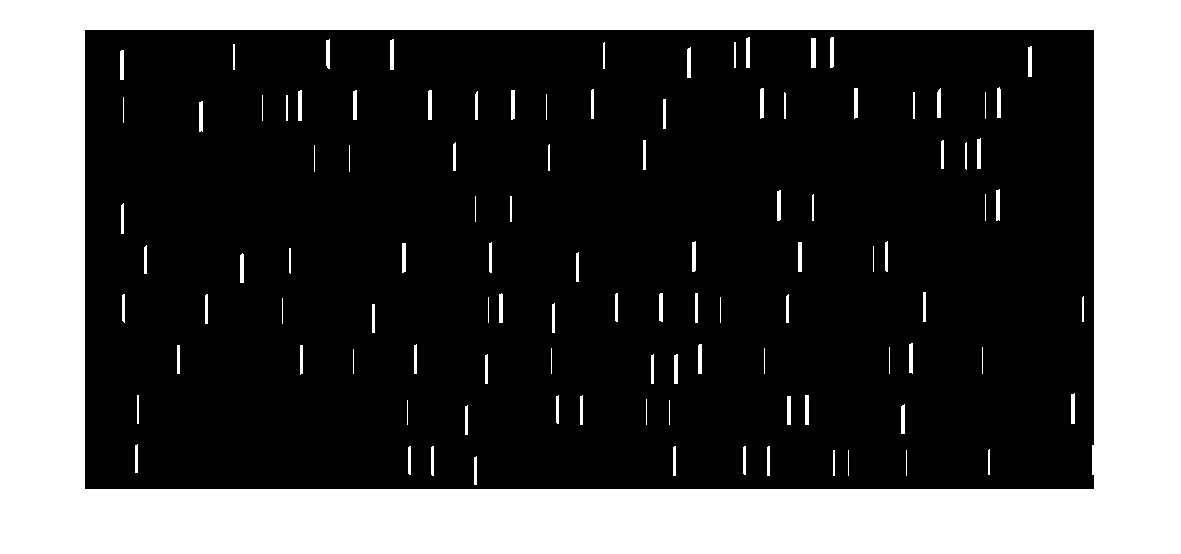
\includegraphics[width=\linewidth]{myfigure/p8/fig0929(c).png}
		\caption{}
		\label{fig:0929c}
	\end{subfigure}
	\begin{subfigure}[b]{0.45\linewidth}
    	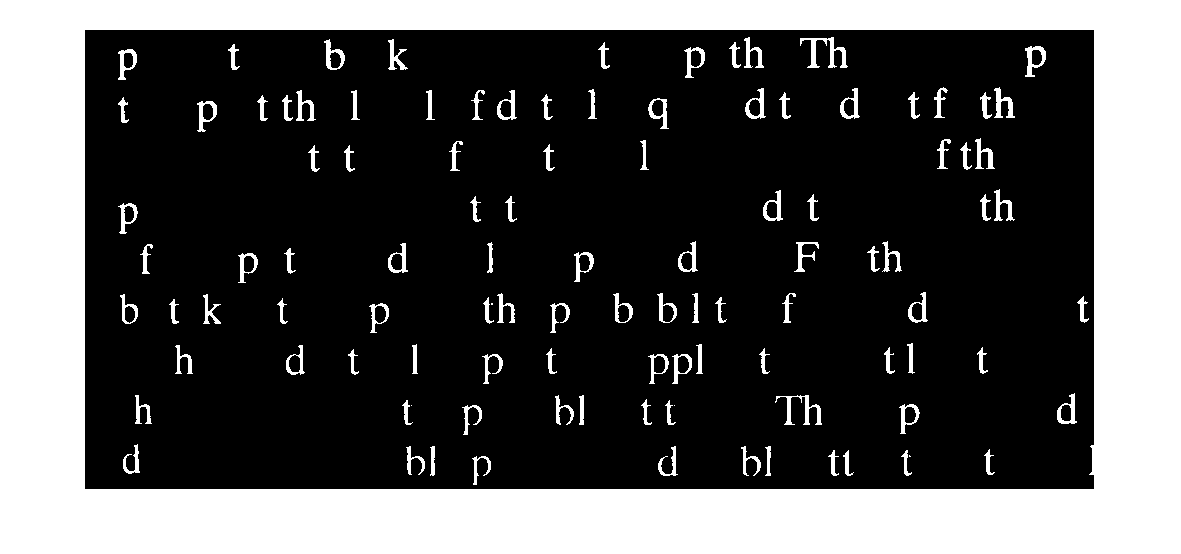
\includegraphics[width=\linewidth]{myfigure/p8/fig0929(d).png}
    	\caption{}
    	\label{fig:0929d}
  	\end{subfigure}
  	\caption{Task1-opening by reconstruction. (a)Original binary image $918 \times 2018$. (b)Erosion of (a) with a structuring element of size $51 \times 1$ pixels. (c)Opening of(a) with the structuring element $51 \times 1$, shown for comparison. (d)Result of opening by reconstruction.}
  	\label{fig:0929}
\end{figure}

The size of geodesic dilation reconstruction is $76$. This process cost about $7$ minutes. I output some of the intermediate results in Figure \ref{fig:0929append} that help us understand the reconstruction better.
\begin{figure}
	\centering
	\begin{subfigure}[b]{0.45\linewidth}
		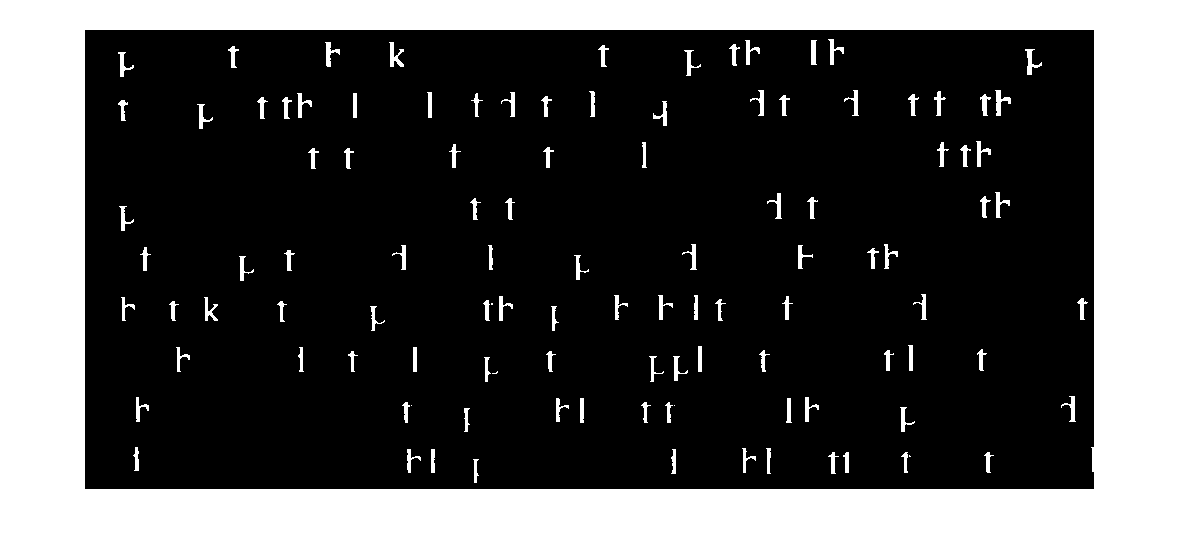
\includegraphics[width=\linewidth]{myfigure/p8/fig0929(d20).png}
		\caption{}
		\label{fig:0929d20}
	\end{subfigure}
	\begin{subfigure}[b]{0.45\linewidth}
    	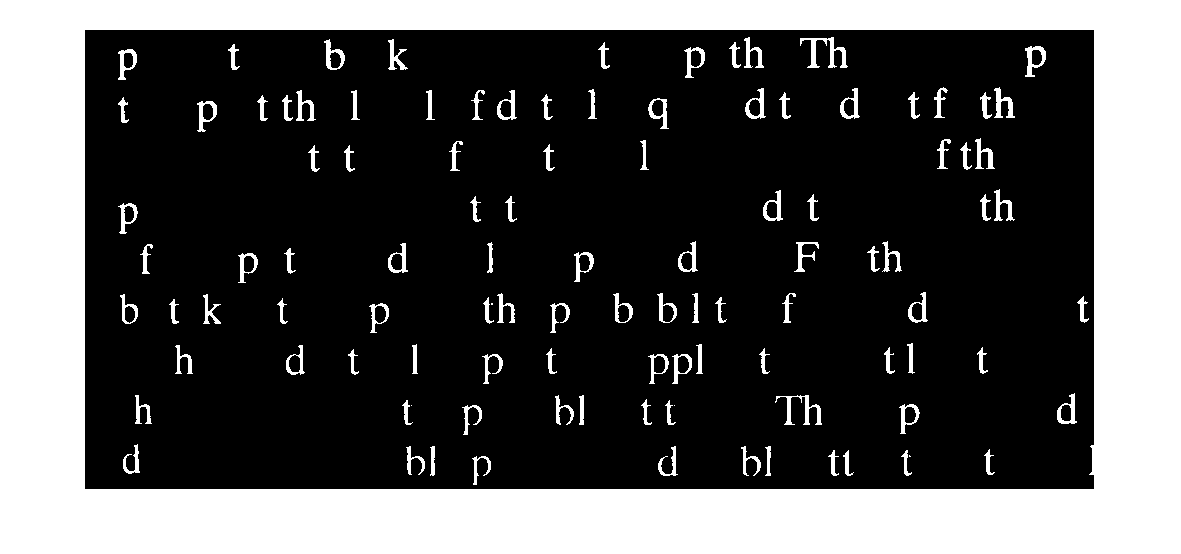
\includegraphics[width=\linewidth]{myfigure/p8/fig0929(d).png}
    	\caption{}
    	\label{fig:0929d76}
  	\end{subfigure}
	\caption{See task-1's process in details. (a)Dilation of size $20$. (b)Dilation of size $76$, the final results.}
  	\label{fig:0929append}
\end{figure}


\subsection{Task-2 Hole filling}
Here we develop a fully automated procedure based on morphological reconstruction. Let $I(x,y)$ denote a binary image and we form a marker $F$ that is $0$ everywhere, except at the image border; that is,
\begin{equation}
F(x, y)=\left\{
\begin{array}{rcl}
1-I(x,y) & \text{if $(x,y)$ is on the border of $I$} \\
0 & \text{otherwise} 
\end{array} \right.
\end{equation}
Then \begin{equation} H=\left[ R_{I^c}^D(F) \right]^c \end{equation} is a binary image equal to $I$ with all holes filled. \\
I use $3\time 3$ structuring element. The hole filling images are shown in Figure \ref{fig:0931}. A detailed process of dilation reconstruction with intermediate results are shown in Figure \ref{fig:0931append}. The reconstruction takes $479$ steps of dilation, which costs a very long period of about $40$ minutes. 
\begin{figure}[h!]
	\centering
	\begin{subfigure}[b]{0.45\linewidth}
		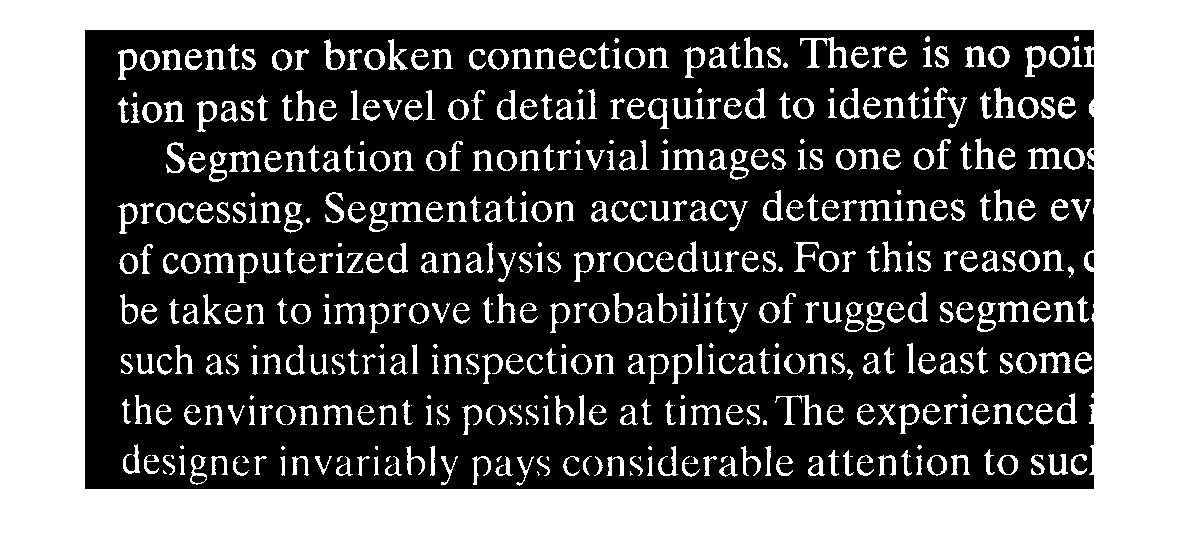
\includegraphics[width=\linewidth]{myfigure/p8/fig0929(a).png}
		\caption{}
		\label{fig:0931a}
	\end{subfigure}
	\begin{subfigure}[b]{0.45\linewidth}
    	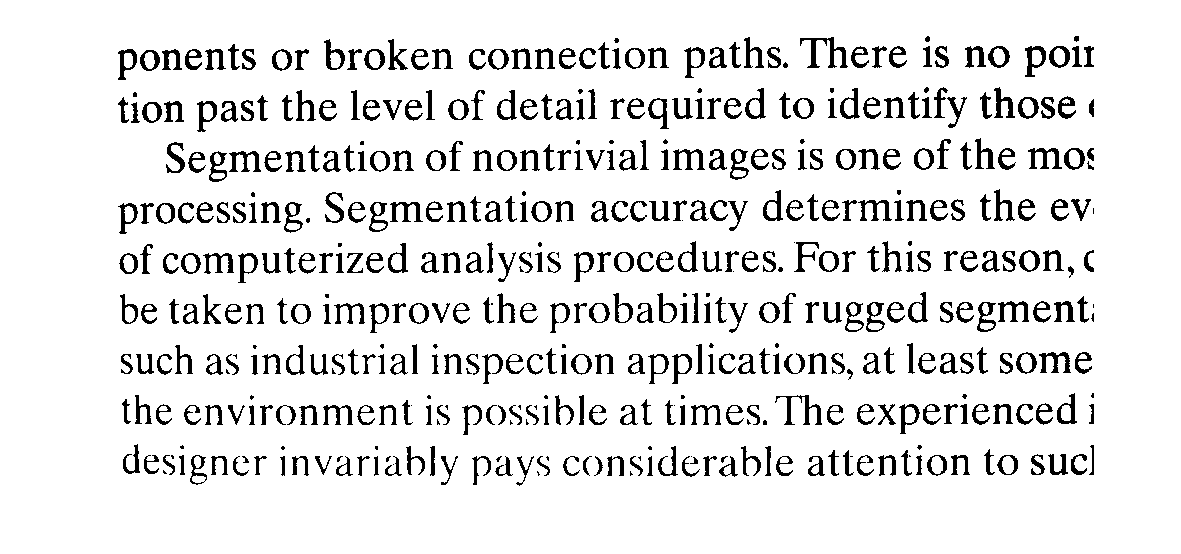
\includegraphics[width=\linewidth]{myfigure/p8/fig0931(b).png}
    	\caption{}
    	\label{fig:0931b}
  	\end{subfigure}
  	\begin{subfigure}[b]{0.45\linewidth}
		
\includegraphics[width=\linewidth]{myfigure/p8/fig0931(c).png}
		\caption{}
		\label{fig:0931c}
	\end{subfigure}
	\begin{subfigure}[b]{0.45\linewidth}
    	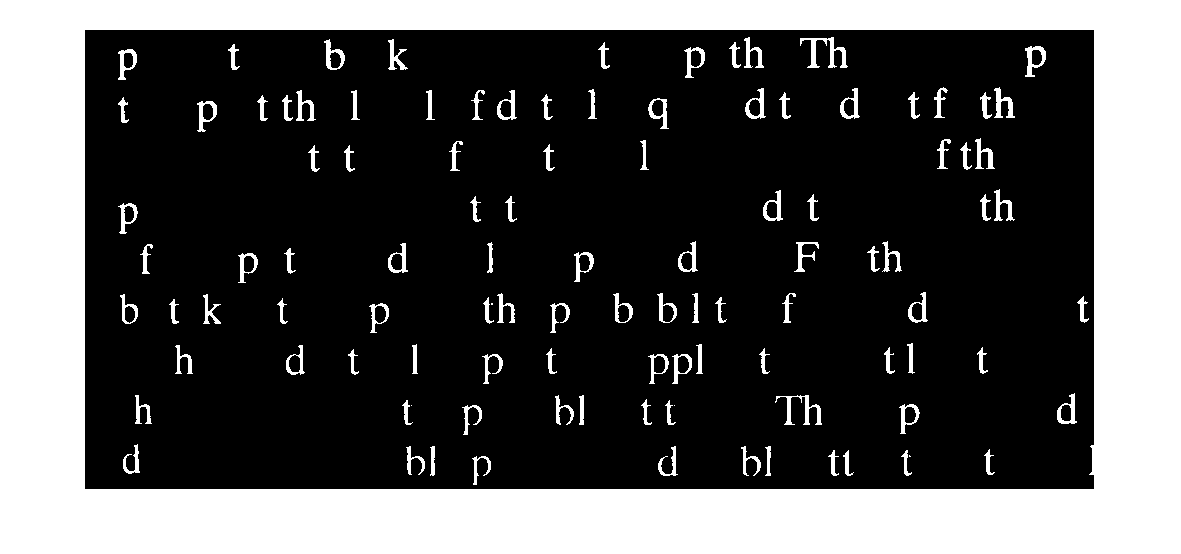
\includegraphics[width=\linewidth]{myfigure/p8/fig0929(d).png}
    	\caption{}
    	\label{fig:0931d}
  	\end{subfigure}
  	\caption{Task2-hole filling. (a)Original binary image $918 \times 2018$. (b)Complement of (a). Used as a mask. (c)Marker image. Seems like a whole black one, but in fact with some white on border. (d)Result of opening by reconstruction.}
  	\label{fig:0931}
\end{figure}

\begin{figure}[h!]
	\centering
	\begin{subfigure}[b]{0.45\linewidth}
		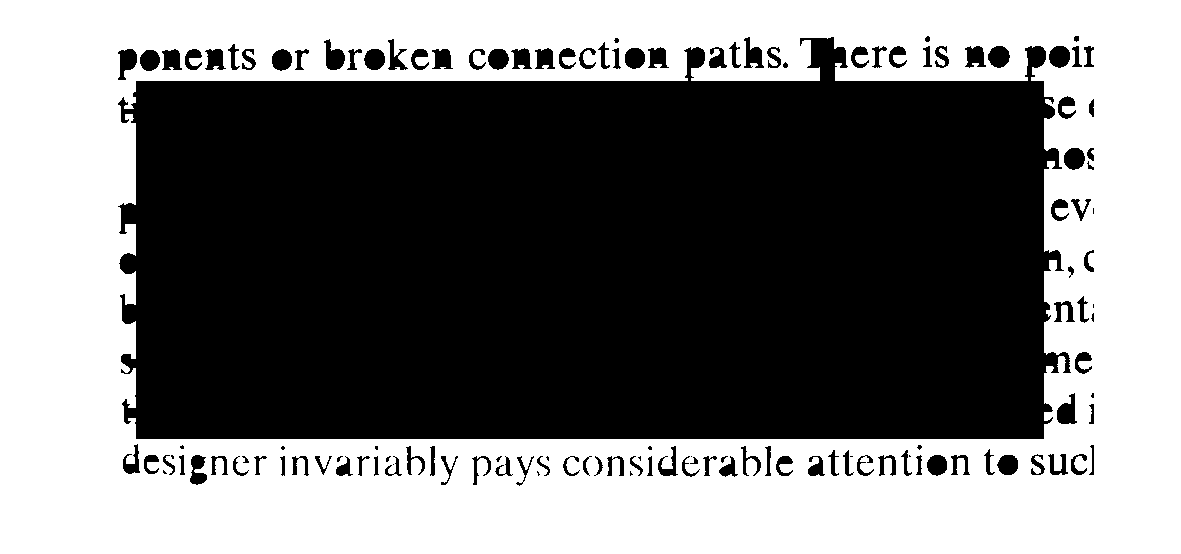
\includegraphics[width=\linewidth]{myfigure/p8/fig0931(d100).png}
		\caption{}
		\label{fig:0931d100}
	\end{subfigure}
	\begin{subfigure}[b]{0.45\linewidth}
    	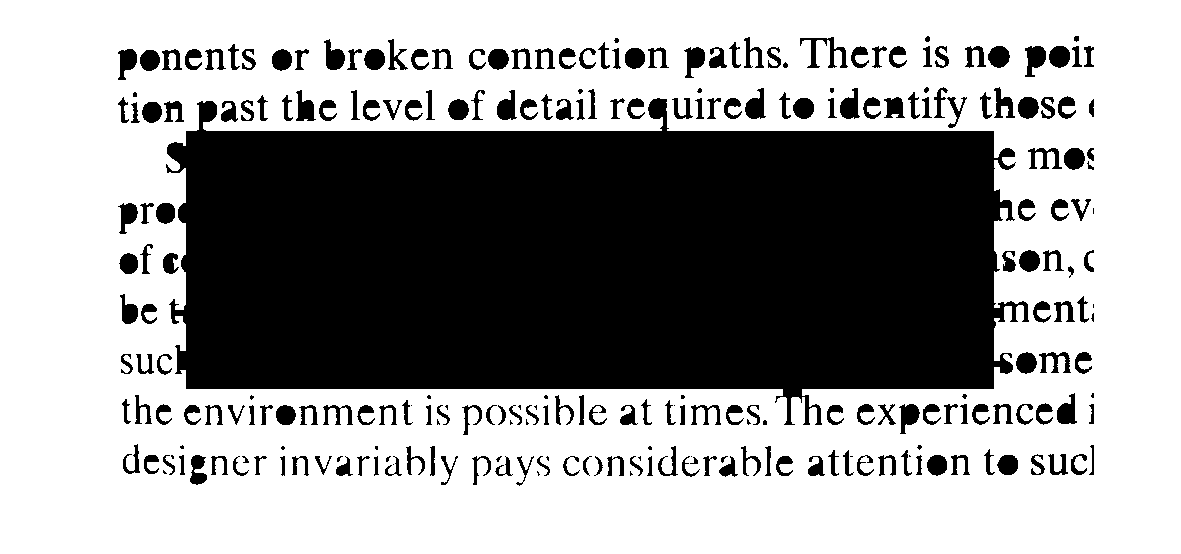
\includegraphics[width=\linewidth]{myfigure/p8/fig0931(d200).png}
    	\caption{}
    	\label{fig:0931d200}
  	\end{subfigure}
  	\begin{subfigure}[b]{0.45\linewidth}
		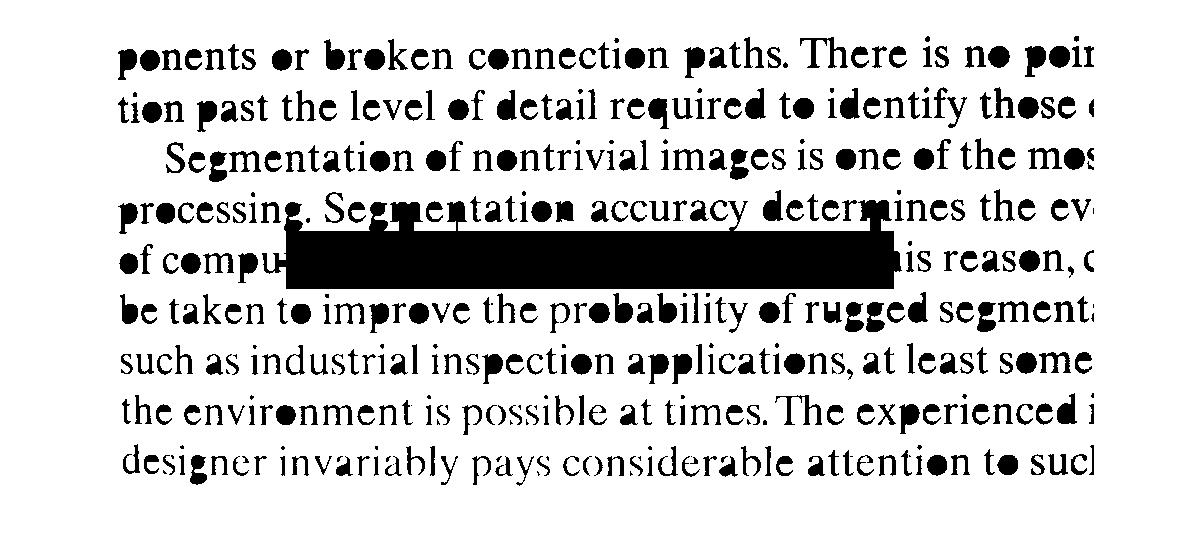
\includegraphics[width=\linewidth]{myfigure/p8/fig0931(d400).png}
		\caption{}
		\label{fig:0931d400}
	\end{subfigure}
	\begin{subfigure}[b]{0.45\linewidth}
    	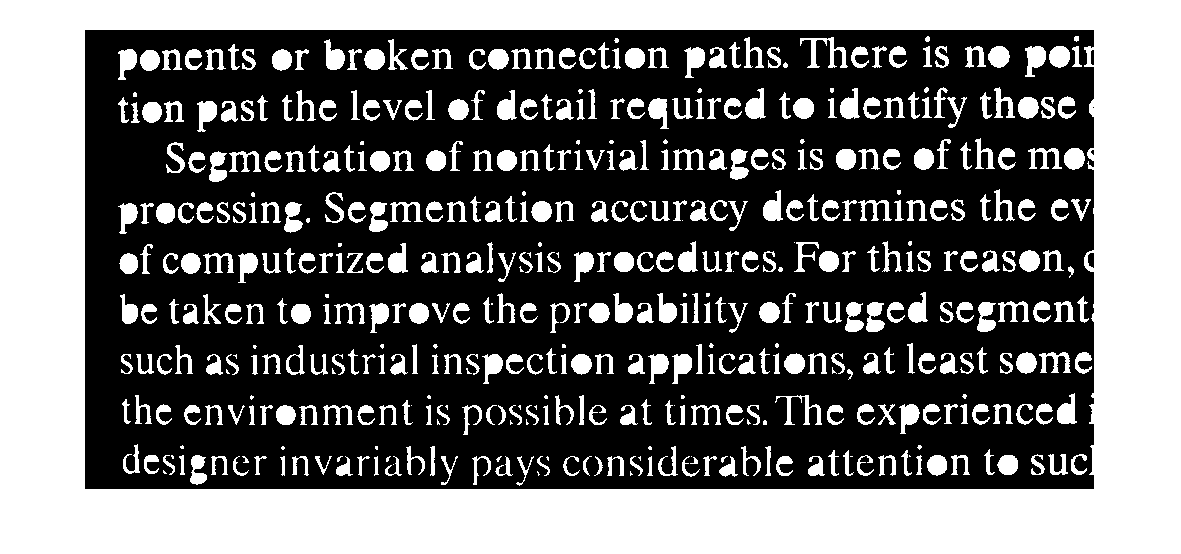
\includegraphics[width=\linewidth]{myfigure/p8/fig0931(d).png}
    	\caption{}
    	\label{fig:0931d479}
  	\end{subfigure}
  	\caption{The process of hole filling in details. (a)After 100 steps of dilation. (b)After 200 steps of dilation. (c)After 400 steps of dilation. Much closer to success! (d)The final result with completion.}
  	\label{fig:0931append}
\end{figure}


\subsection{Task-3 Border clearing}
Removing objects that touch the border is a useful work because it can screen images so that only complete objects remain for further processing. The marker $F(x,y)$ is defined as:
\begin{equation}  
F(x, y)=\left\{
\begin{array}{rcl}
I(x,y) & \text{if $(x,y)$ is on the border of $I$} \\
0 & \text{otherwise} \\
\end{array} \right.
\end{equation}
First we computes morphological reconstruction $R_I^D(F)$ and then computes the desired image $X$
\begin{equation} X=I-R_I^D(F) \end{equation}
I use structuring element of size $3 \times 3$. This task is much easier than task 2 and takes just $21$ steps of dilation in about $2$ minutes. Results are shown in Figure \ref{fig:0932}.
\begin{figure}[h!]
	\centering
  	\begin{subfigure}[b]{0.45\linewidth}
		
\includegraphics[width=\linewidth]{myfigure/p8/fig0932(a).png}
		\caption{}
		\label{fig:0932a}
	\end{subfigure}
	\begin{subfigure}[b]{0.45\linewidth}
    	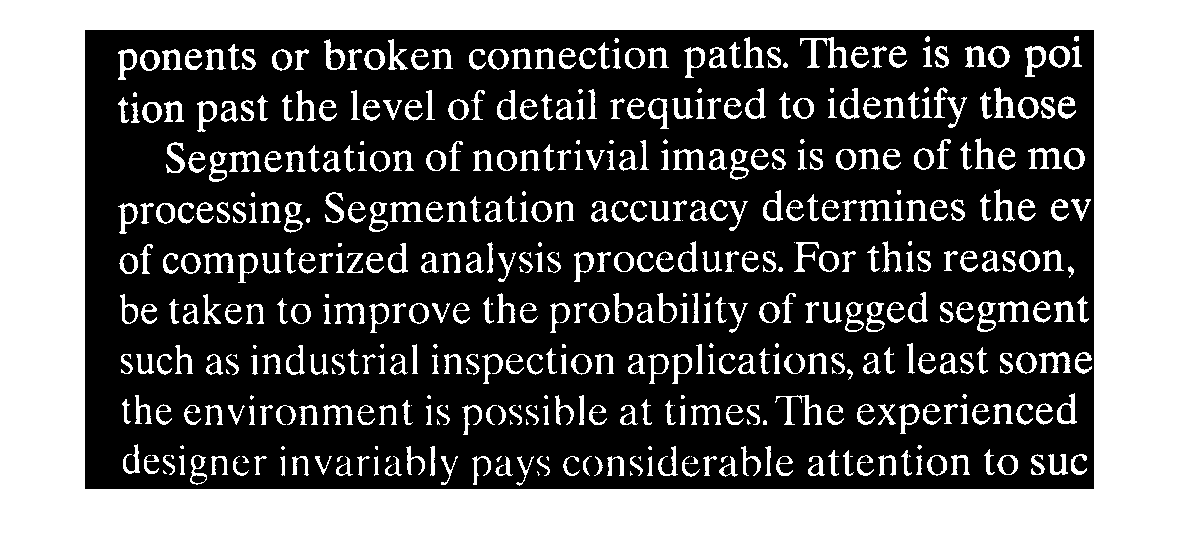
\includegraphics[width=\linewidth]{myfigure/p8/fig0932(b).png}
    	\caption{}
    	\label{fig:0932b}
  	\end{subfigure}
  	\caption{Border clearing. (a)After use border marker for 21-dilation reconstruction. The border letter. (b)The final result after subtraction.}
  	\label{fig:0932}
\end{figure}

\subsection{Implementation}
Matlab functions \emph{erosion, dilation, geodesic\_dilation, dilation\_reconstruction and opening\_reconstruction} are implemented for this project. I made a \textbf{mistake} on opening\_reconstruction at first that I still use $51 \times 1$ as the maker while calling dilation\_reconstruction. The wrong output image is the same as (c) as all the shorter horizontal adjacent relationship in our wanted characters was damaged. So for correction, we must use $3 \times 3$ as structuring element for dilation\_reconstruction called in opening\_reconstruction. \\
In the below code frame, I list the key part of these functions. Other process of calling these functions in main script are trivial so omitted here.\\
\lstset{language=Matlab}
\begin{lstlisting}
% key part of function erosion
for i = (1:M-m+1)
    for j = (1:N-n+1)
        x = imgf(i:i+m-1, j:j+n-1);
        if sum(sum(x.*B)) == m*n
            g(i+downshift, j+rightshift) = 1;
        end
    end
end

% key part of dilation_reconstruction 
k_times = 0;
while( ~isequal(f0, f1) )
    k_times = k_times + 1;
    f0 = f1;
    f1 = geodesic_dilation(f1, G, B);
end

% key part of geodesic_dilation
imgg = dilation(imgf, B) & G;

% key part of opening_reconstruction
for i=(1:n_size)
    f_erosion = erosion(f_erosion, B);
end
[imgg, k_times] = dilation_reconstruction(f_erosion, imgf, ones(3,3)); % here can not use ones(51, 1)
\end{lstlisting}

\subsection{Discussion}
These three tasks show the basic idea of morphological reconstruction used in feature extraction. We start from a marker which can be  obtained easily. Then we use the mask as the constrain to conduct set operations. More advanced topics are morphological operations on gray intensity images and image segmentation. This is a very interesting subproject.
The main obstacle here is \textbf{time}! I tried to do much vectorization but still have a big problem that 20-step-dilation cost about 2 minutes on the $918\times 2018$ image but the complexity is only about $918 \times 2018 \times 20 \times 9 \approx 4 \times 10^8$. I think the computation of this complexity need no more than 2 sec on language like C++ or python. However, I tried the matlab toolbox \emph{IPT} and it's just as fast as the expectation (within 2 sec). This is a strange but interesting problem.


\end{document}